\section{静电场中的导体}

\subsection{静电平衡}

将不带电的导体放入静电场 $\vect{E}_0$，导体内部的自由电子会再电场作用下移动。移动的电荷会产生感应电场 $\vect{E}'$。直到导体内部 $\vect{E}_0 + \vect{E}' = \vect{0}$，导体达到经典平衡。

达到经典平衡的导体，内部电场为 $0$。

\subsection{静电平衡下导体的性质}

\subsubsection{尖端放电}

导体静电平衡状态下，电荷都分布在表面，并且曲率越大的位置电荷密度越高，表面电场强度越高。

当电场强度达到阈值时，就出出现放电现象。

\subsubsection{导体空腔}

对于一个空心导体，内表面的感应电场会抵消内部电场，外表面的感应电场会抵消外部电场。因此内部和外部的电场不会相互影响。

这就是静电屏蔽。

\section{作业}

\begin{problem}
	习题 1.19
	\begin{solution}
		\begin{enumerate}
			\item[\textbf{1)}] $C$ 处电势为 $\varphi_C = \frac{q}{4 \pi \varepsilon_0 l} + \frac{-q}{4 \pi \varepsilon_0 l} = 0$，$E$ 处电势为 $\varphi_E = \frac{q}{4 \pi \varepsilon_0 \cdot 3l} + \frac{-q}{4 \pi \varepsilon_0 l} = -\frac{q}{6 \pi \varepsilon_0 l}$。电场做功和路径无关，因此：
			$$
			W = q_0 (\varphi_C - \varphi_E) = \frac{q q_0}{6 \pi \varepsilon_0 l}
			$$

			\item[\textbf{2)}] 无穷远处电势 $\varphi_{\infty} = 0$。因此做功：
			$$
			W = -q_0 (\varphi_E - 0) = \frac{q q_0}{6 \pi \varepsilon_0 l}
			$$
		\end{enumerate}
	\end{solution}
\end{problem}

\begin{problem}
	习题 1.21
	\begin{solution}
		直接根据电势叠加原理进行积分：
		$$
		\begin{aligned}
			U(x) & = \frac{Q}{2\pi R^2} \cdot \frac{1}{4 \pi \varepsilon_0} \cdot \int_{0}^{2\pi} \int_{0}^{R} \frac{1}{\sqrt{r^2 + x^2}} \cdot r \dd{\theta} \dd{r} \\
			& = \frac{Q}{4 \pi \varepsilon_0 R^2} \int_{0}^{R} \frac{r \dd{r}}{\sqrt{r^2 + x^2}} \\
			& = \frac{Q}{4 \pi \varepsilon_0 R^2} \int_{0}^{R} \frac{\dd(r^2)}{2 \sqrt{r^2 + x^2}} \\
			& = \frac{Q}{4 \pi \varepsilon_0 R^2} \ab(\sqrt{R^2 + x^2} - \abs{x})
		\end{aligned}
		$$

		图像如下：
		\begin{figure}[H]
			\centering
			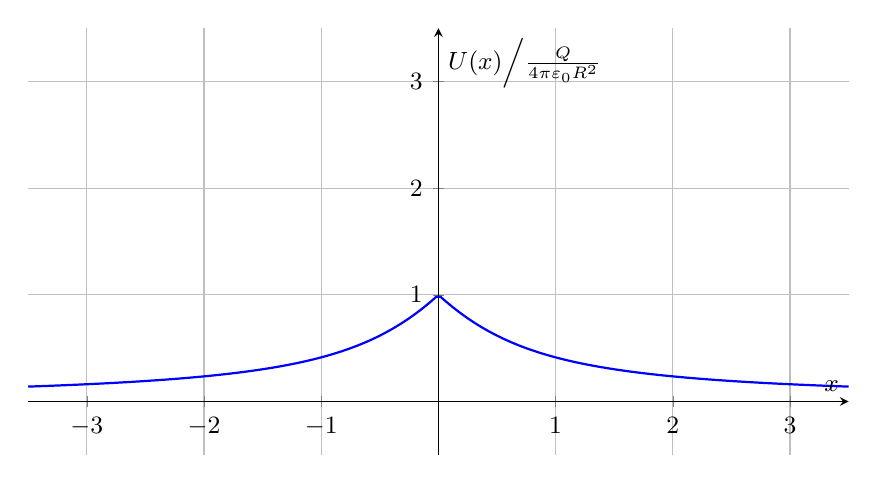
\begin{tikzpicture}
				\begin{axis}[
					xlabel={$x$},
					ylabel={$U(x)\Big/\frac{Q}{4 \pi \varepsilon_0 R^2}$},
					domain=-3.5:3.5,
					samples=200,
					grid=major,
					width=12cm,
					height=7cm,
					legend pos=north east,
					xtick={-3,-2,...,3},
					ytick={0,1,...,3},
					ymin=-0.5,
					ymax=3.5,
					restrict y to domain=0:10,
					axis lines=middle,
					label style={font=\small},
					tick label style={font=\small},
				]
					\addplot[thick, blue] {sqrt(1 + x^2) - abs(x)};
				\end{axis}
			\end{tikzpicture}
			\caption{$U(x)$ 的图像}
		\end{figure}
	\end{solution}
\end{problem}

\begin{problem}
	习题 1.22
	\begin{solution}
		利用 Gauss 定律，取半径 $R$ 处的一个无限长圆筒作为高斯面，得到场强：
		$$
		E(r) = \frac{\lambda_1}{\varepsilon_0} \cdot \frac{1}{2 \pi r} = \frac{\lambda_1}{2 \pi \varepsilon_0 r}
		$$
		因此电势为：
		$$
		\varphi(r) = \int_{r}^{R_2} R(t) \dd{t} = \frac{\lambda_1}{2\pi \varepsilon_0} \ln \frac{R_2}{r}
		$$
	\end{solution}
\end{problem}

\begin{problem}
	习题 1.23
	\begin{solution}
		对于一个半径为 $R$，电荷面密度 $\sigma$ 的完整均匀带电球面，其内部场强为 $0$，因此电势相等，为表面电势：
		$$
		\varphi = \frac{4 \pi R^2 \sigma}{4 \pi \varepsilon_0 R} = \frac{\sigma R}{\varepsilon_0}
		$$
		完整球面内部电势可由两个半球面叠加得到，而两个半球面电势贡献相等。因此，一个半球面，在底面处产生的电势是 $\varphi$ 的一半，即
		$$
		\varphi' = \frac{\sigma R}{2 \varepsilon_0}
		$$

		回到原题，根据电势叠加原理，得到：
		$$
		\varphi(r) = \begin{dcases}
			\frac{\sigma_1 R_1 + \sigma_2 R_2}{2 \varepsilon_0} &,\ r < R_2 \\
			\frac{\sigma_1 R_1}{2 \varepsilon_0} &,\ R_2 \le r < R_1 \\
		\end{dcases}
		$$
	\end{solution}
\end{problem}

\begin{problem}
	习题 1.24
	\begin{solution}
		电离能数值上等于电子的电势能绝对值，即：
		$$
		E = \frac{e^2}{4 \pi \varepsilon_0 r} \approx 2.18 \times 10^{-18} \,\mathrm{J} \approx 13.6 \,\mathrm{eV}
		$$
	\end{solution}
\end{problem}

\begin{problem}
	习题 1.25
	\begin{solution}
		对于单个电荷线密度为 $\eta$ 的导线，距离 $r$ 处的场强为：
		$$
		E(r) = \frac{\eta}{\varepsilon_0} \cdot \frac{1}{2 \pi r} = \frac{\eta}{2 \pi \varepsilon_0 r}
		$$
		因此距离 $r$ 处的电势为：
		$$
		\varphi(r) = \int_{r}^{r_0} E(t) \dd{t} = \frac{\eta}{2 \pi \varepsilon_0} \ln \frac{r_0}{r}
		$$

		来到原题，取 $r_0 = a$，那么：
		$$
		\varphi(x, y) = \frac{\eta}{2\pi \varepsilon_0} \ln \frac{a}{\sqrt{(x - a)^2 + y^2}} - \frac{\eta}{2\pi \varepsilon_0} \ln \frac{a}{\sqrt{(x + a)^2 + y^2}} = \frac{\eta}{2\pi \varepsilon_0} \ln \sqrt{\frac{(x + a)^2 + y^2}{(x - a)^2 + y^2}}
		$$
	\end{solution}
\end{problem}